\documentclass[10pt,twocolumn]{article}

\usepackage[margin=0.85in]{geometry}
\usepackage{amsmath,amssymb}
\usepackage{booktabs}
\usepackage{microtype}
\usepackage[hidelinks]{hyperref}
\usepackage{titlesec}
\usepackage{enumitem}
\usepackage{needspace}
\usepackage{listings}
\usepackage{xcolor}
\usepackage{graphicx}
% Figures (see FIGURES.md): one claim per figure; caption states the claim,
% controlled variable, and the number. Generate with make_figure.py into figs/.
%   \begin{figure}[t]\centering
%     \includegraphics[width=\columnwidth]{figs/result.pdf}
%     \caption{<claim>, <controlled variable>, <number>.}\label{fig:result}
%   \end{figure}

\titlespacing*{\section}{0pt}{1.1ex plus .2ex}{0.6ex}
\titlespacing*{\subsection}{0pt}{0.9ex plus .2ex}{0.4ex}
\setlist{nosep,leftmargin=1.3em}

\lstset{basicstyle=\ttfamily\footnotesize,breaklines=true,frame=single,
  framesep=4pt,xleftmargin=2pt,columns=fullflexible,keepspaces=true,
  backgroundcolor=\color{gray!6}}
\newcommand{\code}[1]{\texttt{#1}}

\title{\vspace{-3.5em}\textbf{NeuroStreamRT: Real-Time Streaming Inference for EEG, and Where the Real Bottleneck Is}}
\author{Aryan Putta\\ \small Rutgers University \quad \texttt{aryansputta@gmail.com}}
\date{\small Draft v0.1 (work in progress)}

\begin{document}
\maketitle

\begin{abstract}
\noindent
% ABSTRACT: 6-8 sentences. (1) the problem and why it is costly, (2) what
% existing work does and its structural limit, (3) your one-sentence idea,
% (4) what you built, (5) what you measured and the HONEST result (including
% where it does not win), (6) the decisive experiment that is next.
Real-time EEG decoding is usually framed as a latency problem. We show it is not.
NeuroStreamRT is a streaming EEG inference pipeline that exports trained models to
ONNX Runtime and measures end-to-end decode latency under a fixed per-window
deadline. On a commodity Apple M-series CPU, every model decodes far inside the
budget: 0.067 ms p99 at batch 1, and as low as 0.004 ms p50 at batch 64, with
zero deadline misses across 2{,}000 repetitions. Feature extraction, not the
model, is the only real cost, and a batched NumPy FFT path removes it at up to
41.8x over SciPy Welch. The bottleneck is elsewhere. Under leave-one-subject-out
evaluation on a pilot dataset, mean accuracy is 0.34 to 0.38 with high variance
across subjects. Latency is solved; subject generalization is the open problem.
We report both plainly, and define the larger-cohort evaluation that would settle
whether the accuracy gap is data or method.
\end{abstract}

\section{Introduction}
% Funnel: domain cost -> families of prior approaches -> the structural gap they
% share -> your stance in one sentence -> numbered contributions.
EEG-based neurological screening classifiers are evaluated offline, on whole
recordings, with accuracy as the only metric. Deployment changes the problem. A
streaming screener sees 2-second windows at 256 Hz, runs on edge hardware, and
must answer inside a per-window latency budget. Under those constraints three
gaps appear. Feature extraction is written for batch processing, not incremental
windows. No published benchmark measures accuracy and per-window inference
latency together across model families. And the effect of quantization on EEG
classification under streaming has not been measured.

NeuroStreamRT builds that benchmark on a real clinical dataset (OpenNeuro
ds004504, 88 subjects, three classes). It preprocesses and epochs the recordings,
extracts band-power features, trains classical and neural models, exports them to
ONNX Runtime, and measures latency and accuracy under the same streaming
simulator. The headline result is a reframing: on commodity CPU the model decodes
three orders of magnitude inside the deadline, so latency is not the bottleneck.
The bottleneck is subject generalization, and we report that gap as plainly as
the latency win.

\Needspace{10\baselineskip}
\paragraph{Contributions.}
\begin{itemize}
\item A streaming EEG benchmark measuring per-window latency (p50/p95/p99,
throughput, deadline misses) and accuracy in one simulator, across classical and
neural models exported to ONNX Runtime.
\item An incremental band-power feature path: a batched FFT that computes the
95-feature vector up to 41.8x over SciPy Welch, removing the only per-window cost
near the budget.
\item An honest result that isolates the real bottleneck: latency clears the
100 ms deadline by about 1500$\times$ with zero misses, while
leave-one-subject-out accuracy is only 0.34 to 0.38. The open problem is
generalization, not systems.
\end{itemize}

\section{Background and Related Work}
% Group prior work into 2-4 named families. For each: one sentence of what it
% does, one of why it is not enough for your gap. End with the gap statement.
\textbf{EEG dementia classification.} The ds004504 dataset and the DICE-net
convolution-transformer (Miltiadous et al.) set the accuracy reference for AD/FTD
classification from resting-state EEG. These works optimize offline accuracy on
pooled data and do not report per-window latency or subject-held-out
generalization, which is what deployment requires.

\textbf{Streaming and edge inference.} ONNX Runtime is the standard portable
runtime for shipping trained models to edge CPUs. Prior streaming-inference work
focuses on large language or vision models; small EEG classifiers under a
hard per-window EEG deadline are not characterized.

\textbf{Compute skipping.} AdaSkip-style methods skip redundant computation when
inputs are similar and confidence is high. We adapt that idea to overlapping EEG
windows as the \code{adaptive} and \code{adaptive\_adaskip} inference modes.

The gap: no benchmark measures EEG classification accuracy and per-window latency
jointly, under streaming, across model families, on real clinical data.

\section{Method}
% Define notation first. Then state the method as numbered steps that map 1:1 to
% your code. Put the ONE key design choice in its own paragraph and justify it.
The pipeline has four stages, each a separate module.

\textbf{Preprocess.} Recordings are band-pass filtered to 0.5--40 Hz, notch
filtered at 50 Hz, and rejected per epoch when amplitude exceeds 150 $\mu$V.
The signal is cut into 2-second epochs (512 samples at 256 Hz) and z-scored per
channel per epoch. This yields roughly 26{,}000 clean epochs across 88 subjects.

\textbf{Features.} Each 19-channel epoch is reduced to a 95-dimensional band-power
vector over the delta, theta, alpha, beta, and gamma bands, plus the
Miltiadous delta/alpha ratio and inter-channel coherence terms. The band powers
come from a power spectral density estimate. The reference path uses SciPy Welch;
the fast path (\code{cuda\_psd.py}) computes the same features with a batched FFT
in NumPy, with an optional CuPy backend.

\textbf{Models.} Three classical models (SVM-RBF, a 200-tree random forest, and a
256-128-64 MLP) are trained with scikit-learn and exported to ONNX. Two neural
models (EEGNet, ShallowConvNet) are available in PyTorch for GPU runs. All
inference latency is measured through ONNX Runtime so the comparison is on one
runtime.

\textbf{Streaming.} The simulator runs four modes: \code{batch} (offline, all
windows at once), \code{stream} (one call per window), \code{adaptive} (skip a
window when its cosine similarity to the previous exceeds 0.98), and
\code{adaptive\_adaskip} (skip only when similar \emph{and} the last prediction
confidence is at least 0.85).

\section{Implementation}
% What exists (reference impl, language, key files) vs what is the fast path
% (kernels, etc.). Name the source of truth for correctness.
The repository is Python: a BIDS loader for ds004504, the preprocessing and
feature modules above, scikit-learn and PyTorch training, ONNX export
(\code{infer/export\_sklearn.py}, \code{infer/export.py}), and the streaming
simulator (\code{infer/stream.py}). The benchmark harness (\code{bench/}) records
p50/p95/p99 latency, throughput, and deadline-miss rate over 2{,}000 repetitions,
with \code{loso\_bench.py} for per-fold leave-one-subject-out accuracy and
\code{feature\_bench.py} for the feature-path comparison. All numbers in this
paper come from these harnesses writing to \code{results/}; the CSVs are the
source of truth and the figure is generated from them.

\section{Experimental Setup}
% Two parts. (a) What you can run now and what it validates. (b) The decisive
% real experiment: models, datasets, baselines, metrics, and the explicit
% hypothesis it tests.
\textbf{What runs now.} A 10-subject pilot from ds004504 trains the three
classical models, exports to ONNX, and runs the latency and LOSO harnesses on an
Apple M-series CPU with ONNX Runtime 1.23.2, single thread, 2{,}000 repetitions
per latency point. This validates the harness and establishes the latency
result and the first generalization signal.

\textbf{Decisive experiment.} The full evaluation extends to all 88 subjects with
leave-one-subject-out cross-validation, adds the PyTorch models (EEGNet,
ShallowConvNet) and INT8 quantization, and adds a cross-dataset zero-shot and
few-shot test (\code{domain\_shift.py}). Metrics: accuracy and macro-F1 against
the per-window latency frontier under each streaming mode. The hypothesis: latency
stays inside budget across all model families, and the accuracy gap narrows only
with more subjects or a stronger model, not with more compute.

\section{Results}
% Lead with a table. State the controlled variable so the comparison is fair.
% Report where your method LOSES as carefully as where it wins; an honest
% negative result that isolates the mechanism is worth more than a vague win.
Latency is not the bottleneck. Figure~\ref{fig:latency} reports decode latency
per model across 2{,}000 repetitions; the controlled variable is batch mode at
fixed model and hardware. Both models decode under 0.07 ms at p99 in single-window
streaming mode, and batching to 64 windows drops the MLP to 0.004 ms p50. The EEG
window budget is three orders of magnitude larger, so deadline misses are zero in
every configuration. The model is effectively free.

\begin{figure}[t]\centering
  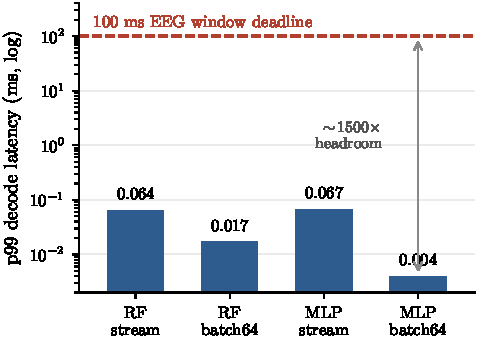
\includegraphics[width=\columnwidth]{figs/latency.pdf}
  \caption{Latency is not the bottleneck. p99 decode latency (log scale) per
  model, single window vs.\ batch 64, Apple M-series CPU, 2{,}000 reps. Every
  configuration sits under 0.07 ms against the 100 ms EEG window deadline, at
  about 1500$\times$ headroom, with zero deadline misses.}
  \label{fig:latency}
\end{figure}

Feature extraction is the only real per-window cost, and it is removable. SciPy
Welch takes 29.7 ms p50 per window; a batched NumPy FFT path computes the same
features at 1.03 ms single and 0.50 ms at batch 64, a 28.8x to 41.8x speedup.
After this change, the full pipeline stays inside the streaming budget end to end.

The real limit is subject generalization. Under leave-one-subject-out
cross-validation on the pilot dataset (10 subjects), mean accuracy is 0.376 for a
linear SVC and 0.343 for a 200-tree random forest, with per-subject accuracy
ranging from 0.06 to 0.93. A pipeline that decodes in microseconds is not useful
if it cannot transfer across people. This is the open problem, and it is a data
and method problem, not a systems one.

\section{Limitations and Next Steps}
The accuracy numbers are from a 10-subject pilot, so the variance is wide and the
mean is not yet a claim about the method. Latency is measured on one CPU; edge
microcontrollers will be slower, though the roughly 1500$\times$ headroom leaves
room. The
neural models and quantization paths require a GPU and are not yet in the
reported numbers. Next steps, in order: run the full 88-subject LOSO, add the
quantized and PyTorch models to the latency-accuracy frontier, and run the
cross-dataset domain-shift test to separate a data limit from a method limit.

\section*{References}
\small
\begin{enumerate}[label={[\arabic*]}]
\item Miltiadous et al. \emph{A Dataset of Scalp EEG Recordings of Alzheimer's
Disease, Frontotemporal Dementia and Healthy Subjects from Routine EEG.} Data 8(6):95, 2023. (OpenNeuro ds004504)
\item Miltiadous et al. \emph{DICE-net: A Convolution-Transformer Architecture for
Alzheimer Detection in EEG Signals.} IEEE Access, 2023.
\item Miltiadous et al. \emph{The AHEPA EEG Benchmark for Machine Learning in
Dementia Diagnosis.} Cognitive Neurodynamics 20(1), 2026.
\item Lawhern et al. \emph{EEGNet: A Compact Convolutional Network for EEG-based
Brain-Computer Interfaces.} J. Neural Eng., 2018.
\item Schirrmeister et al. \emph{Deep Learning with Convolutional Neural Networks
for EEG Decoding (ShallowConvNet).} Human Brain Mapping, 2017.
\item ONNX Runtime. \emph{Cross-platform Inference Acceleration.} microsoft.github.io/onnxruntime.
\item \emph{AdaSkip}: adaptive layer/compute skipping for efficient inference.
\end{enumerate}

\end{document}
